%  after submission
%
% 
%
%
%
%
%
%
\documentclass{llncs} %
%\documentclass{article}
%\usepackage{natbib}
\usepackage{booktabs}
\usepackage{pslatex}
\usepackage{apacite}
\usepackage{url}
\usepackage{graphicx}
\usepackage{listings}
\usepackage{color}
\usepackage{textcomp}
\usepackage{amsmath}
\usepackage{amssymb}
\usepackage{wrapfig}
\usepackage{lipsum}

 \newcommand{\denote}[1]{\mbox{ $[\![ #1 ]\!]$}}

\definecolor{Red}{RGB}{255,0,0}
\newcommand{\red}[1]{\textcolor{Red}{#1}}  

\newcommand{\subsubsubsection}[1]{{\em #1}}
\newcommand{\eref}[1]{(\ref{#1})}
\newcommand{\tableref}[1]{Table \ref{#1}}
\newcommand{\figref}[1]{Figure \ref{#1}}
\newcommand{\appref}[1]{Appendix \ref{#1}}
\newcommand{\sectionref}[1]{Section \ref{#1}}

\lstset{
  language=Scheme, % Andreas Stuhlm�ller. Scheme listings. https://github.com/stuhlmueller/scheme-listings.git
  columns=fixed,
  tabsize=2,
  extendedchars=true,
  breaklines=true,
  frame=single,
%  numbers=left,
  numbersep=5pt,
    basicstyle=\scriptsize\ttfamily
%  rulesepcolor=\color{solarized@base03},
%  numberstyle=\tiny\color{solarized@base01},
%  keywordstyle=\color{solarized@green},
%  stringstyle=\color{solarized@cyan}\ttfamily,
%  identifierstyle=\color{blue},
%  commentstyle=\color{solarized@base01},
%  emphstyle=\color{solarized@red}
}

\title{Understanding \emph{belief bias} by measuring prior beliefs for a Bayesian model of syllogistic reasoning}

\author{}
%\author{{\large \bf Michael Henry Tessler} (mtessler@stanford.edu)}
\institute{} %Department of Psychology, Stanford University}
 
\begin{document}

\maketitle


\begin{abstract}
Belief bias in syllogistic reasoning is an effect wherein the a priori believability of the conclusion influences the intuitive acceptability of that conclusion \cite{Evans1983}. Prior beliefs about the world can be formalized into a probabilistic generative model of situations. \citeA{Tessler2014} proposed that this very idea can account for the range of acceptability observed across categorical syllogisms with abstract content. Here, I extend their model to accommodate syllogistic reasoning data where content effects are observed. I collect data about the prior plausibility of various properties co-occurring, and use this data to predict syllogistic reasoning behavior in a separate experiment. I compare models with different types of assumptions about the prior and discuss open questions for this approach. 
\end{abstract}

Prior beliefs about the world guide our actions, thoughts, and reasoning in new situations. It can be helpful, for example, to know how fast a particular kind of animal can run, if you are also thinking about if that animal can eat you. Similarly, humans can use prior beliefs in a domain (e.g. life expectancies) to reason about everyday contexts  (e.g. guessing how long someone will live) \cite{Griffiths2006}. Finally, it has been argued that prior beliefs influence the very meaning of words \cite{GoodLass2015}. It is odd then that so little formal theory has gone into understanding prior beliefs in reasoning tasks that have occupied much of cognitive psychology (but, cf. \citeA{Klauer2000, Dube2010}). 

One formal approach, with the potential to model the influence of prior beliefs in syllogistic reasoning, was proposed by \citeA{Tessler2014}, who argued that syllogistic reasoning could be understood through the broader lens of language understanding. This intuition was formalized in a probabilistic model of pragmatic reasoning about syllogistic premises. They found that a probabilistic model of argument strength based on situations populated by objects with properties accounted for much of the variability in conclusion endorsements for syllogisms. That work further explored syllogistic reasoning by incorporating Gricean principles---formalized in the Rational Speech-Act (RSA) theory of language understanding \cite{Frank2012,Goodman2013}---and specifying the Question Under Discussion as the relationship between the conclusion terms (i.e. the QUD is the syllogistic conclusion). This component was important in capturing some of the qualitative phenomena in syllogistic reasoning. %(e.g. the relative preference for the \emph{all X are Y} conclusion over the \emph{some X are Y} conclusion when both are valid).
Here, I extend the model of argument strength to capture qualitative phenomena associated with \emph{belief bias} by incorporating prior beliefs about real-world content and test it against behavioral data obtained in targeted studies of the role of prior beliefs in syllogistic reasoning.

%The extent to which beliefs influence reasoning depends on the a priori acceptability of the conclusion \cite{Evans1983}, of the premises \cite{Cherubini1998}, as well as the relative strength of the argument \cite{Evans2001}. The approach outlined in this paper is to account for the gradience in argument strength in terms of the prior distribution over properties in question; i.e., I explain relative argument strength and the influence of beliefs jointly.

%\subsection{Forward summary}

%In this paper, I address two questions: Does the prior distribution matter for syllogistic reasoning about real world content? Is it necessary to model dependencies in background knowledge? 

The organization for the rest of the paper is as follows. First, I review the model by \citeA{Tessler2014} and propose an extension to account for reasoning about real-world content. I then collect data measuring the prior distributions of various properties co-occurring in 4 domains: frozen fruit, expired crackers, bright lightbulbs, and sharp knives. I also collect data about 8 syllogisms using each domain's content (32 items in total). I then compare the model to the data by integrating out the parameters of the computational model and comparing alternative models with increasingly relaxed assumptions about background knowledge. I conclude by discussing intriguing questions raised by this work.


% \citeA{Evans1999} conducted a standard syllogistic reasoning study (syllogistic reasoning with only abstract terms) and found gradient endorsement rates for logically invalid syllogisms; this gradient can be interpreted as relatively weaker and stronger arguments. \citeA{Evans2001} replicated this finding and found that weaker syllogisms were more susceptible to positive belief bias (i.e. accepting a believable conclusion) and stronger syllogisms were more susceptible to negative belief belief (i.e. rejecting an unbelievable conclusion). This work suggests a gradient influence of prior beliefs on argument strength. 



%\section{Empirical work on syllogistic reasoning}
%
%Syllogistic reasoning lies at the intriguing intersection of logic and language. On the one hand, syllogisms are logical: Indeed, for about two millennia, they comprised the core of formal logic\footnote{By inventing the syllogistic argument, Aristotle incidentally invented \emph{the variable} as well. The fact that a logical form that can be instantiated by literally any content is what makes this bridge to our modern notion of a variable.}. On the other hand, syllogisms are a part of language: Aristotle's logic can be thought of as an early stab at natural language semantics, though there have been considerable improvements since (e.g. \citeA{Horn1989}). Syllogisms are an intriguing intermediate form: Abstract and logically consistent while approachable by any language user. And though as a formal reasoning tool, syllogisms are internally valid and complete, their reliance upon natural language makes them perfectly vulnerable to all of the uncertainty that comes with understanding natural language (for one perspective on uncertainty in language, see \citeA{GoodLass2015}).
%
%\subsection{The syllogistic space}
%
%The syllogism is a logical form: a two-sentence argument used to relate two properties (or terms: A, C) via a middle term (B). In categorical syllogisms (the focus of this paper), the relation between the terms is a quantifier acting on sets. Here is an example of a formal syllogistic argument.
%\begin{quote}
%Premise 1: All A are B\\
%Premise 2: Some B are C\\
%Conclusion: Some A are C
%\end{quote}
%The full space of syllogistic arguments (64 premise pairs in total) is derived by shuffling the ordering of the terms in a premise (``All A are B'' vs. ``All B are A'') and changing the quantifier (\emph{all, some, none, not all}). Most syllogisms are invalid, i.e. the conclusion (i.e. the relation between terms A \& C) is not true in every situation in which the premises are true. For example, the argument above is invalid. Participants, however, are perfectly comfortable drawing a conclusion. A recent meta-analysis of syllogistic reasoning showed that over the population, the ``false alarm'' rate for a invalid syllogisms ranged from 24\% to 88\%. For valid arguments, the accuracy for a \emph{logically valid conclusion} ranged from 1\% to 90\% \cite{Khemlani2012}. Such heterogeneity in accuracy for logical valid responses suggests a computational-level theory based on deductive validity is untenable. 

%\subsection{Prior beliefs in syllogistic reasoning}
%
%The divergence between human reasoning and deductive logic is probably why syllogistic reasoning has been a topic of interest for a long time \cite{Storring1908,Woodworth1935, Chapman1959, JL1978, Chater1999}. Many factors affect the acceptability of a syllogistic conclusion. One very prominent factor is the content of the syllogistic argument. For example, \citeA{Wilkins1928} observed that
%
%\begin{quote}
%No A are B\\
%No B are C\\
%Therefore, no A are C
%\end{quote}
%
%produced appreciably fewer endorsements than 
%
%\begin{quote}
%No apples are oranges\\
%No oranges are lemons\\
%Therefore, no apples are lemons
%\end{quote}
%
%In more targeted studies since, it's been consistently shown that the \emph{a priori} believability of the conclusion influences the acceptability of the conclusion. This was first characterized as an interaction between logic and belief \cite{Evans1983}. It may not be only the believability of the \emph{conclusion} that influences reasoning, however. \citeA{Cherubini1998} found the a priori believability of the \emph{premises}, too, is relevant factor in determining what conclusions to draw from an argument. 

%\citeA{Evans1983} demonstrated that the \emph{a priori} believability of the conclusion influences the acceptability of the conclusion, and that this influence was more pronounced for invalid rather than valid syllogisms. This characterization of this interplay between logic and belief has been debated \cite{Newstead1993, others}.  For example, when experimenters have included neutral materials for baseline comparisons, they find belief bias is primarily associated with \emph{rejecting unbelievable} conclusions particularly when the syllogism is invalid, leading some investigators to refer to it as ``belief debias'' \cite{Morley2004, Newstead1992}.

%The extent to which beliefs influence reasoning also seems to depend on the relative strength of the argument. \citeA{Evans1999} conducted a standard syllogistic reasoning study (syllogistic reasoning with only abstract terms) and found gradient endorsement rates for logically invalid syllogisms; this gradient can be interpreted as relatively weaker and stronger arguments. \citeA{Evans2001} replicated this finding and found that weaker syllogisms were more susceptible to positive belief bias (i.e. accepting a believable conclusion) and stronger syllogisms were more susceptible to negative belief belief (i.e. rejecting an unbelievable conclusion). This work suggests a gradient influence of prior beliefs on argument strength. 
%
%\subsection{Forward summary}
%
%In this paper, I address two questions: Does the prior distribution matter for syllogistic reasoning about real world content? Is it necessary to model dependencies in background knowledge? 
%
%The organization for the rest of the paper is as follows. First, I review the model by \citeA{Tessler2014} and propose an extension to account for reasoning about real-world content. I then collect data measuring the prior distributions of various properties co-occurring in 4 domains: frozen fruit, expired crackers, bright lightbulbs, and sharp knives. I also collect data about 8 syllogisms using each domain's content (32 items in total). I then compare the model to the data by integrating out the parameters of the computational model and comparing alternative models using Bayesian data analytic techniques. I explore the predictions of the inferred ``best model'' and discuss future predictions. 

% Next, I plug these priors into the Bayesian model of argument strength to generate predictions for all 64 syllogisms. I compare these predictions with predictions of a model of argument strength that uses i.i.d. priors. Critically, this model will not predict content effects. I compare the predictions for the two models using a newly developed technique for optimal experiment design (OED). In Experiment 1, I collect data from 4 syllogisms are that highly ranked in the OED analysis. I compare the models and show that that the empirically elicited prior beliefs as the prior distribution for the argument strength model is the better account of the data from Experiment 1. 
%
%I then go on to investigate the interaction of pragmatics with background knowledge. I run the same OED analysis on the full pragmatics model of \citeA{Tessler2014} that uses the empirically elicited prior beliefs versus one that used \emph{i.i.d.} priors. In Experiment 2, I collect data from 4 new syllogisms that are highly ranked in the OED analysis. I compare the models and show that a strong prediction of the full pragmatics model with background knowledge is \emph{not} born out. This leads to a reconsideration of the generative model of the situations. In particular, I reflect on the recent findings of \citeA{Degen2015} that listeners reconsider world knowledge when utterances are odd. I revisit the full pragmatics model with these findings in mind, and reanalyze the data from Experiment 1 and 2. I find that the pragmatics model that is sensitive to the \emph{a priori} plausibility of the syllogism given the empirically elicited prior beliefs matches the data from Experiments 1 \& 2 the best. I end with a discussion of the implications of this model for the belief bias literature broadly. 



\section{Bayesian argument strength in syllogistic reasoning}

Gradience in syllogistic reasoning was formalized by \citeA{Tessler2014} (henceforth, TG). The computational model presented by TG is a Bayesian model; as such, it is important to understand the implications of the prior for syllogistic reasoning. The model samples situations which are composed of objects with properties. 

Situations are composed of $n$ objects:
\begin{lstlisting}
(define objects (list 'o1 'o2 ... 'on))
\end{lstlisting}

(Ellipses indicate omissions for brevity, otherwise models are specified via runnable Church\footnote{The model was written in the probabilistic programming language Church \cite{probmods}, a higher-order probabilistic logic based on the lambda calculus. For background and details on this form of model representation, see \url{http://probmods.org}} code\footnote{A fully-specified version of this model can be accessed at: \url{http://forestdb.org/models/syllogisms-cogsci14.html}}.) Properties \lstinline{A}, \lstinline{B}, and \lstinline{C} of these objects are represented as functions from objects to the property value. Properties are assumed to be Boolean. The TG model assumed no a priori information about the meaning of the properties; thus, properties were determined independently and identically:

\begin{lstlisting}
(define A (mem (lambda (x) (flip br))))
(define B (mem (lambda (x) (flip br))))
(define C (mem (lambda (x) (flip br))))
\end{lstlisting}

Note that the operator \lstinline{mem} memoizes these functions, so that a given object has the same value each time it is examined within a given situation, even though it is initially determined probabilistically (via \lstinline{flip}\footnote{For clarity, \lstinline{(flip br)} is equivalent to Bernoulli ($br$).}). Hence, the number of objects $n$ is a parameter of the model, as is the base rate $P(x)=br$ of properties. In fitting the model to the meta-analysis data by \citeA{Chater1999}, TG found $P(x) \sim 0.25$. This is qualitatively consistent with the ``rarity assumption'' --- that properties are relatively rare of objects --- first used by \citeA{Oaksford1994}.

The Bayesian model has a very natural way to account for prior beliefs in reasoning. Indeed, beliefs simply specify a different prior distribution of properties. In particular, the assumption that properties are \emph{independent and identically distributed (\emph{i.i.d.}} must be relaxed if we are to consider real-world content. I extend the model by considering that properties can follow any discrete distribution; the presence or absence of properties can be represented by the joint distribution $P(a,b,c)$:

\begin{lstlisting}
(define ABC (mem (lambda (x) 
     (multinomial (list 'ABC 'AB_ 'A_C '_BC 'A__ '_B_ '__C '___) real-world-prior))))
\end{lstlisting}


%\subsection{Model overview and previous findings}
%
%The Bayesian model has two structural aspects to it: first, there is the computation of argument strength. This is done by computing by $P(conclusion | premises)$ by way of the \emph{situations} described above. Argument strength was shown to capture much of the quantitative variance in the syllogistic reasoning meta-analysis data.
%
%The second structural component is pragmatic, recursive reasoning about the relevance of the premises for each conclusion. This works by considering not just the strength of the syllogistic argument at hand, but also the relative strengths of alternative syllogistic arguments that could have been given but weren't. This model component was shown to be sufficient to capture qualitative phenomena that the argument strength alone could not capture. In particular, this model highlighted where deviations from literal semantics interpretation would occur (e.g. the relative preference for an \emph{all} conclusion over a \emph{some} conclusion when both are logically valid). 
%
%In this paper, I am going to consider the role of prior beliefs by focusing of the first of these model components: the generative model of argument strength.

\subsection{A generative model of argument strength}

The model of argument strength relies upon the interpretation of quantifier sentences as truth-functional operators, consistent with standard practice in formal semantics. 


A quantifier (e.g. \lstinline{all}) is a function of two properties (e.g. \lstinline{A} and \lstinline{B}) which maps to a truth value by consulting the properties of the objects in the current situation. For instance:
\begin{lstlisting}
(define all (lambda (A B) 
    (all-true (map (lambda (x) (if (A x) (B x) true)) objects))))
\end{lstlisting}
The function \lstinline{map} applies the given function ---\lstinline{(lambda ...)}--- to each element of the list \lstinline{objects}. The helper function \lstinline{all-true} simply checks that all elements of a list are true, i.e. that all the \emph{As} are indeed \emph{Bs}. In a similar way, \lstinline{some}, \lstinline{none}, \lstinline{not-all} are defined to have their standard meanings. 

The key observation to connect these truth-functional meanings of quantifier expressions to probability distributions over situations is that an expression which assigns a Boolean value to each situation can be used for probabilistic conditioning. That is, these quantifier expressions can be used to update a prior belief distribution over situations to a posterior belief distribution. For syllogistic reasoning, we are interested not in the posterior distribution over situations \emph{per se}, but the distribution on true conclusions that these situations entail. In Church this looks like:
\begin{lstlisting}
(query
 (define objects (list 'o1 'o2 ... 'on))
 . . . define A,B,C . . .
 . . . define all, some, no, not-all . . .
 (define true-conclusions (filter (lambda (conclusion) (conclusion A C))
 								 all-conclusions))

 true-conclusions
 
 (condition	(and (premise-one A B)
      			(premise-two B C))))
\end{lstlisting}

The first arguments to a query function comprise a generative model: the background knowledge with which a reasoning agent is endowed. Definitions for which a prior is stipulated (e.g. \lstinline{A, B, C} i.e, the situation in terms of the properties) denote aspects of the world over which the agent has uncertainty. The second argument, called the \emph{query expression}, is what the agent wants to know. The final argument, called the \emph{conditioner}, is the information with which the agent updates her beliefs; it is what she knows. This model, thus, returns a posterior distribution over conclusions conditioned on some premises being true.



%\begin{eqnarray}
%&&P_{argument-strength}(c|p)\propto \delta_{\denote{p}(x)} \cdot P(c|x)  \cdot P(x)  \label{eq:L0}\\ % not sure about this
%&&P_{experimenter}(p|c) \propto \mathrm{exp}({\lambda \cdot \ln P_{argument-strength}(c|p))}  \label{eq:S1}\\ 
%&&P_{pragmatic-reasoner}(c|p)\propto P_{experimenter}(p|c)\cdot P(c|x)  \cdot P(x)  \label{eq:L1}
%\end{eqnarray}
%
%Here $\denote{p}: X \rightarrow \text{Boolean}$ is a truth-function specifying the literal meaning of each set of premises. This is derived from the 
%usual literal semantics of the 4 syllogistic quantifiers applied to the situations of objects of properties. 
%
%$\denote{p_{\textrm{all of the As are Bs}}}=\forall{x}: A(x) \Rightarrow B(x)$
%
%$\denote{p_{\textrm{some of the As are Bs}}}= \exists{x}: A(x) \Rightarrow B(x)$
%
%$\denote{p_{\textrm{some of the As are not Bs}}}= \exists{x}: A(x) \Rightarrow \neg{B(x)}$
%
%$\denote{p_{\textrm{none of the As are Bs}}}= \forall{x}: A(x) \Rightarrow \neg{B(x)}$
%
%$P(x) = P(a,b,c)$ specifies the prior distribution over situations. For TG, the properties \emph{a, b, c} were assumed to be i.i.d. and hence, $P(x) = P(a, b, c) = P(a)\cdot P(b)\cdot P(c) = P(br)^3$, where \emph{br} was the base rate of properties parameter, which was fit to the data. Here, $P(x) = P(a, b, c)$ which will be measured empirically (Experiment 1). It will be used to make predictions about $P(c|p)$ to model the syllogistic reasoning data (Experiment 2). It is important to consider the joint distribution of properties and not just their respective marginal probabilities because it's likely there will be important correlations among the properties of real-world content.


%
%\section{Experiment 1: Measuring $P(a, b, c)$ for real-world content}
%\label{prelicit}
%
%To achieve reliability of the prior estimates, I selected 4 domains that could be interpreted as having properties with causal relationships because people typically have strong intuitions about causal domains. The 4 causal domains divided into two structural forms: common cause and common effect, in order to increase the variability of the domains. 
%
%\subsubsection{Design}
%
%I recruited 70 participants on Amazon's Mechanical Turk to rate the likelihood of various combinations of properties co-occurring. Participants were paid \$0.80 for their work.
%
%I ran the experiment using two different dependent measures as a between-subjects variable. Each participant was randomly assigned to either the ``frequency'' or the ``plausibility'' dependent measure condition. Within each of these conditions, participants completed the ``frequency'' or ``plausibility'' judgment task for all 4 domains. The design can be summarized as follows: 2 (task: ``frequency'' or ``plausibility'' judgment; between subjects) x 4 (domains: see table \ref{tab:domains}; within subjects).
%
%
%\subsubsection{Procedure \& Materials}
%





%The most reliable way of eliciting probability judgments from subjects remains an open question. We ran the prior elicitation with two different dependent measures to examine the reliability of our materials.
%For each causal structure, we explored relations where the 
%used 3 different domains. 
%
%We based our selection of domains on simulations of argument-strength using qualitatively different priors (elicited from people in the lab). Our simulations suggested that domains using: \red{\{common-cause / multiple-cause\}} with \red{\{2-enabling / 2-preventative / 1-enabling,1-preventative\}} and a conclusion relating \red{\{cause and effect, 2 causes, 2 effects\}} lead to the largest differences between model predictions.
%For each domain, participants were told to either ``Imagine an X (e.g. a lightbulb)'' or ``Imagine 100 Xs'' and told to rate the plausibility or frequency, respectively, of all 8 possible combinations of the presence and absence of the properties found in Table \ref{tab:domains}. Slider bars ranged from ``Impossible'' to ``Certain'' or ``0'' to ``100'', respectively. These different dependent measures were collected to examine the reliability of our materials. Participants rated all 8 combinations of properties for each domain.

%The instructions for the ``plausibility'' condition, were as follows: ``Imagine an X (e.g. a lightbulb; see Table \ref{tab:domains}, column ``Noun''). How likely is it that it:''  The instructions for the ``frequency'' condition were: ``Imagine 100 Xs (e.g. lightbulbs). About how many of them:''
%
%Below these prompts were listed the 8 possible combinations of the presence and absence of the Properties A, B, C found in Table \ref{tab:domains}. In the ``plausibility'' condition, the properties agreed with the singular form of the noun (e.g. ``is on'', ``is bright'', and ``is hot''). In the ``frequency'' condition, properties agreed with the plural form (e.g. ``are on'', ``are bright'', and ``are hot''). All 8 combinations of the presence and absence of properties (``are on, are bright, aren't hot''; ``are on, aren't bright, are hot'', etc...) were listed. Next to each set of properties, was a slider bar.
%
%In the ``plausibility'' condition, the slider bar ranged from ``Impossible'' to ``Certain'', with intermediate arrows pointing to the left and right indicating ``less likely'' and ``more likely''. In the ``frequency'' condition, the slider bar ranged from ``0'' to ``100'', with intermediate arrows pointing to the left and right indicated ``fewer'' and ``more''. 


%\subsubsection{Data analysis and results}
%
%Participants' responses were normalized within each domain so that the ratings for the 8 property combinations made a well-formed probability distribution (i.e. they added up to 1). I then took the mean rating for each of the 8 property combinations in each of the 4 domains, to arrive at mean empirical priors for all 4 domains. These were used as the empirical $P(a,b,c)$ for the Bayesian model. 
%
%The experiment elicited unique priors for each domain (see Figure \ref{fig:priors}). The data elicited with different dependent measures were highly correlated ($r_{pearson} = 0.78; r_{spearman} = 0.85$). I collapsed ratings across dependent measures for use in the Bayesian model\footnote{Though the correlations are good between the prior data elicited by different dependent measures, the correlations were even higher ($r_{pearson} \thicksim 0.95$) between the model predictions based on these different dependent measures.}.






%$P(\delta_{\denote{c}(x)})$ is used because the model of argument strength isn't given a conclusion, but rather \emph{generates} a conclusion according to the prior distribution over situations. $P(\delta_{\denote{c}(x)})$ ensure that a conclusion wihich is true of the 


%For concreteness, assume that the number of objects in a situation is 4. The relevant number of objects that satisfy the a premise will depend on that particular premise. For example, \emph{All of the grey elephants are herbivores} is true if all of the elephants that are grey in the particular situation are also herbivores\footnote{N.B. I use the ``of the'' construction to make clear that I am describing a particular situation of elephants and not elephants in general.}. The model is given some number of elephants: in our example, 4. The model then samples properties \emph{grey, herbivore} according to the joint prior distribution of these properties $P(x) = P(g,h)$. Depending on the prior probabilities of $g$, a given situation may have 0, 1, 2, 3, or 4 grey elephants. The premise that \emph{All of the grey elephants are herbivores} is evaluated with respect to the number of grey elephants in that situation. If there are 3 grey elephants, then $\denote{\emph{All of the grey elephants are herbivores}]}: \forall{x}, g(x) \Rightarrow h(x)$

%and $S = \{s_0, s_1, s_2, \dots, s_{4}\}$, where the subscript indicates the number of objects (e.g., marbles) that exhibit an effect (e.g., sinking). 
%Further assume that the set of utterances \emph{All/None/Some of the marbles sank} is denoted $U = \{u_{\textrm{all}}, u_{\textrm{none}}, u_{\textrm{some}}\}$ and each has its usual literal meaning: 
%%$\denote{u_{\textrm{none}}}: s=0$,  
%%$\denote{u_{\textrm{some}}}: s>0$,
%%$\denote{u_{\textrm{all}}}: s=15$.
%$\denote{u_{\textrm{none}}}= \{s_i | i = 0\}$,  
%$\denote{u_{\textrm{some}}}= \{s_i | i > 0\}$,
%$\denote{u_{\textrm{all}}}= \{s_i | i = 15\}$.
\begin{table}
\centering
\tabcolsep=0.11cm
\begin{tabular}{ |c|c|c|c|c|c }
%\small
\hline
\multicolumn{5}{ |c| }{Experiment 1 Domains} \\
\hline
Noun & Causal relation & Property A & Property B & Property C  \\ \hline
%\multirow{4}{*}{Defenders} & LB & Lucus Radebe \\
crackers & common effect & are soggy & are past expiration date & have lots of flavor  \\ \hline
knives & common effect & are sharp & are rusty & cut well  \\ \hline
lightbulbs & common cause & are on & are bright & are hot  \\ \hline
strawberries & common cause & are in the freezer & are soft & are warm  \\ \hline
\end{tabular}
\caption{Content domains used in experiments.}
\label{tab:domains}
\end{table}


\section{Experiment: Syllogistic reasoning about real world content}


In a preliminary experiment, I recruited 70 participants from Amazon's Mechanical Turk to judge the likelihood of various combinations of properties co-occurring (see Table \ref{tab:domains} for the properties used). The resulting empirical priors from that preliminary experiment are shown in Figure \ref{fig:priors}. 



\begin{figure}
\centering
    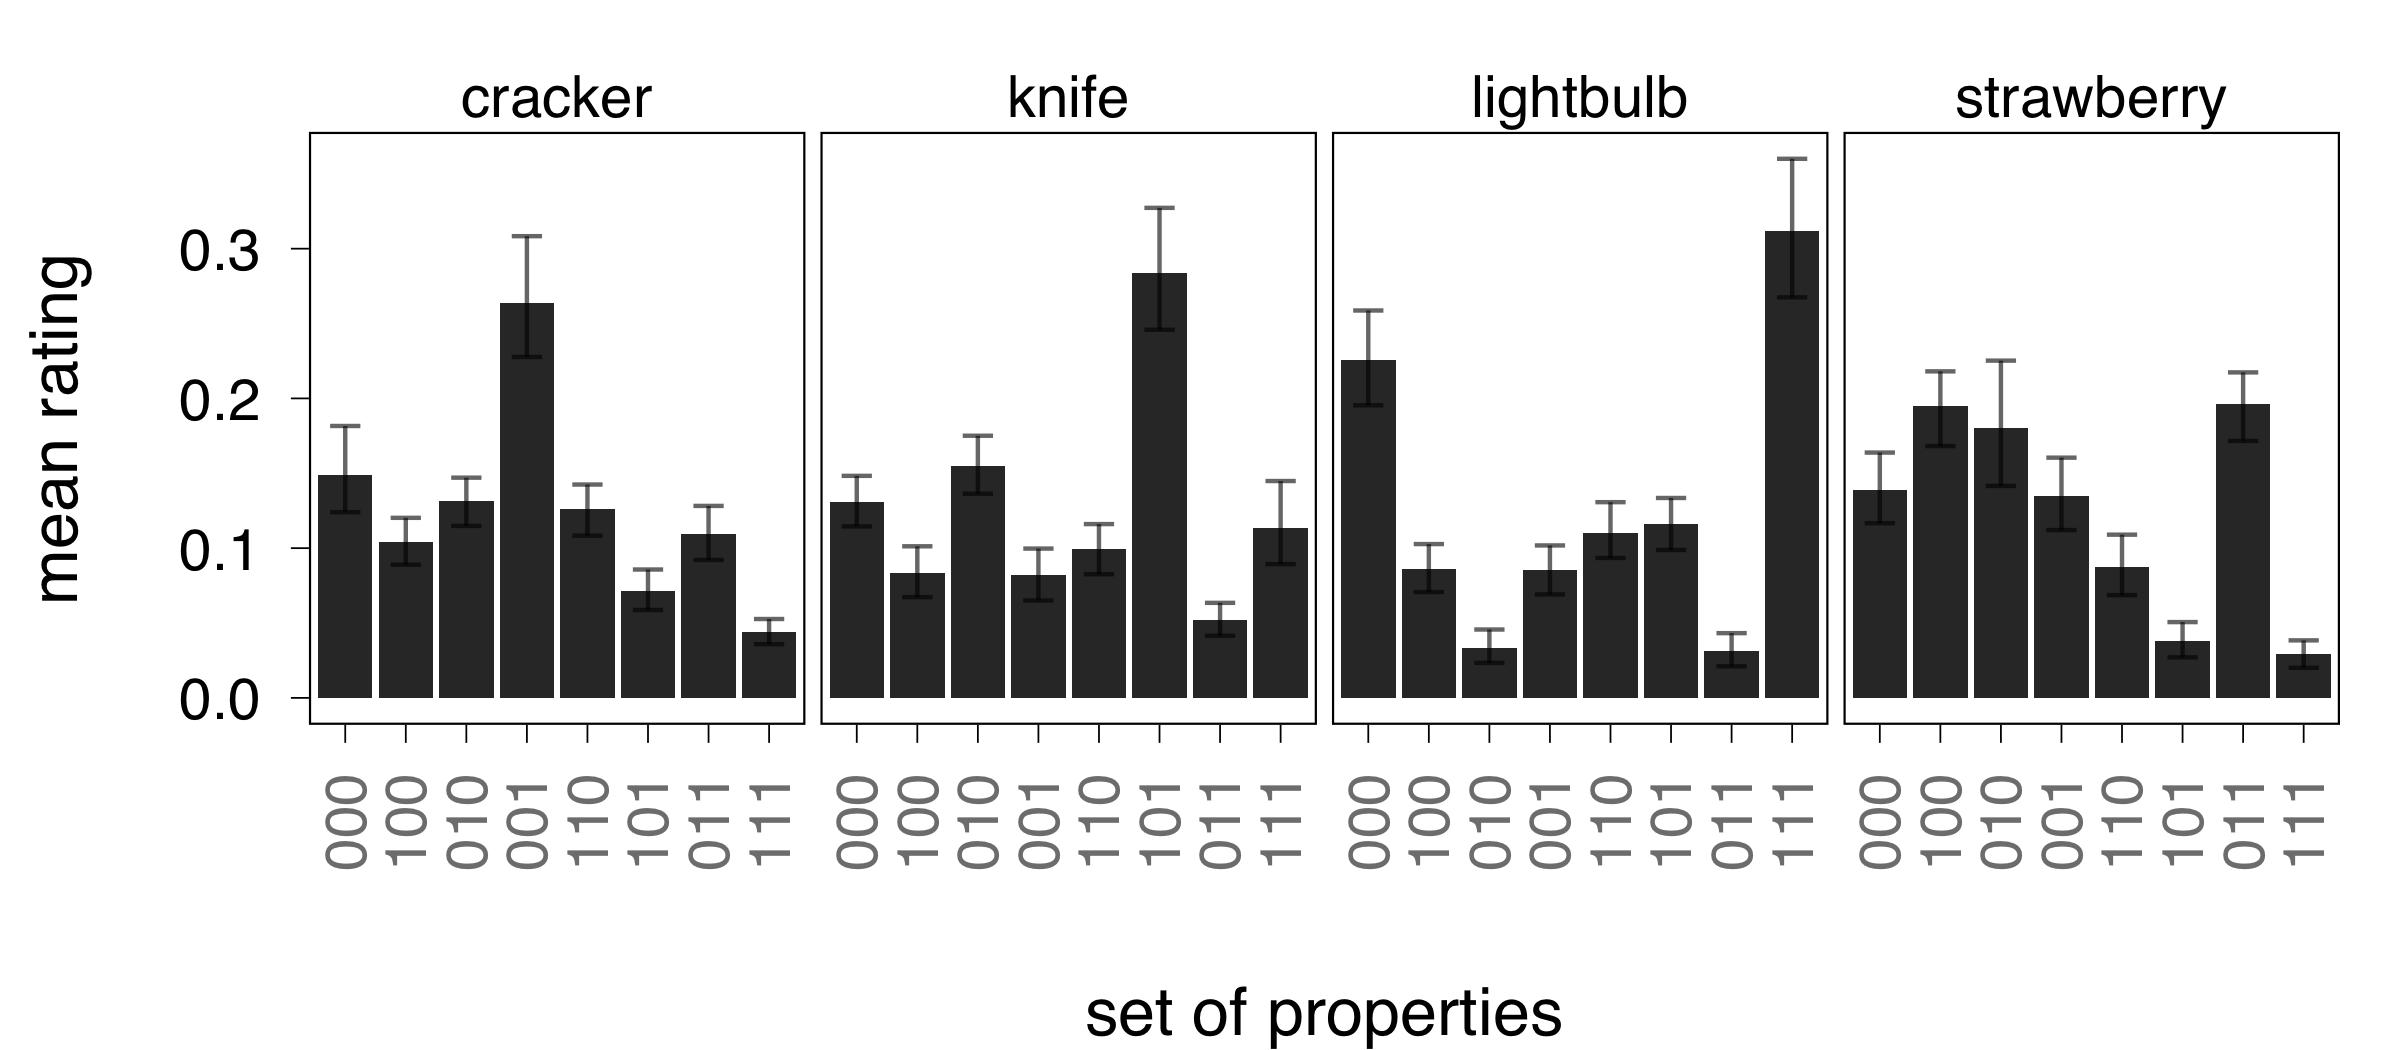
\includegraphics[width=\columnwidth]{priors}
    \caption{Mean elicited priors. X-axis shows presence or absence of each property, the ordering of which can be found in Table \ref{tab:domains}. For example, the tallest bar in the cracker domain (001) is a cracker which isn't soggy, isn't past expiration date, and has lots of flavors.}
  \label{fig:priors}
\end{figure}



I tested if syllogisms using the real world content from the preliminary experiment led to different conclusions.

\subsubsection{Design}

I recruited 254 participants from Amazon's Mechanical Turk. All participants were required to have a 95\% approval rating for their previous work on the web service. Participants were paid \$0.60 for their work. Each syllogism was paired with each domain used in Experiment 1. A total of 8 syllogisms were used, resulting in 32 unique \{syllogism, domain\} pairs.

\subsubsection{Procedures \& Materials}

Each participant completed 4 syllogisms. On each experimental trial, participants were presented with the syllogism (e.g. \emph{Some of the lightbulbs that are bright are on. None of the lightbulbs that are hot are bright.}) and each possible conclusion (e.g. \emph{\{All, Some, Not all, None\} of the lightbulbs that are hot are on.}) and asked ``Does it follow that: X'', for each conclusion. Radio buttons with the options ``Doesn't follow'' and ``Follows'' were provided. Below that was a vertically-oriented slider bar with endpoints labeled ``Certain'' and ``Don't know'' to measure confidence. Participants were required to mark each conclusion before continuing to the next trial.


%\begin{quotation}
%If you think the conclusion follows from the argument, indicate so. Adjust the position of the slider bar to reflect your confidence in your response.
%\end{quotation}


\subsubsection{Results}

Shown in Figure \ref{fig:syllogismXdomain} (darkest bars) are a subset of the results of the experiment. Content effects can be viewed by comparing panels within a row (i.e. comparing across columns). For example, for the \emph{some / none} syllogism (top row), the proportion of responses endorsing  ``Some of the lightbulbs that are hot are on'' is appreciably higher than the proportion endorsing ``Some of the crackers that have lots of flavor are soggy'' (green bars, 2nd row, columns 1 \& 3). Effects of reasoning (i.e. of syllogism) can be observed by comparing panels within a column (i.e comparing down rows). For example, ``Some of the crackers that have lots of flavor are soggy'' is a substantially more endorsed conclusion if the premises are: ``All of the crackers that are past expiration date are soggy. Some of the crackers that have lots of flavor are past expiration date.'' (right column, first and second rows). 

\section{Bayesian analysis of models}

%I compared the predictions of the TG model of argument strength using the priors elicited in the preliminary experiment to the syllogistic reasoning data. 

In this analysis, I explore 4 different models of argument strength that vary in their priors. The first model---the ``abstract'' model---uses a single base-rate parameter in its prior\footnote{This is exactly the model of argument strength used by \citeA{Tessler2014}.}; this model assumes properties are \emph{i.i.d.} both within domains and across domains. The second model---the ``i.i.d'' model---is the simplest parametrized model that can predict content effects; it is identical to the first model except in that the base-rate parameter can vary across domains (but not within a domain). This model has 4 parameters (one for each domain). The third model---the ``independent'' model---assumes only that properties are independent; it uses a different base-rate parameter for each property within and across domains. This model has 12 parameters (3 properties per domain and 4 domains in total). The final model is the model that uses the empirically elicited priors from the preliminary experiment; this model has no free parameters for the prior.

One parameter is shared by all models. This is the number of objects in a situation $n$, which controls how large the worlds are that the reasoner reasons over. A preliminary analysis revealed that results were highly consistent for $n \geq 4$ and so I use $n=4$ for all simulations.  In addition, for all models I include a single data analytic ``guessing'' parameter $\phi \thicksim U(0,1)$ to account for response noise.

%There are two parameters to the model. The first is an optimality or rationality parameter. TG takes the probabilities to represent actual persons in a communicative setting, and so conclusions or premises are selected from these distributions according to a Luce choice, or softmax, decision rule with a parameter $\lambda$ that denotes the degree to which utterances are chosen optimally \cite{Luce1959}. This is one of the parameters of the model. 
%
%I put a uniform prior over the optimality parameter $\lambda \thicksim U(0,5)$.

\begin{figure}
\centering
    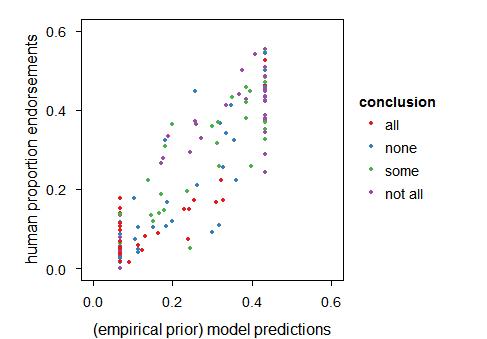
\includegraphics[width=0.5\columnwidth]{figures/scatter}
    \caption{Data vs. (Empirical prior) Model plot. The model provides a good overall fit ($r=0.87$) to the 128 data points (32 syllogism, domain pairs X 4 conclusions each). The posterior predictions bottom out around 0.07. This is the work of the response noise parameter $\phi$. It's likely that different syllogisms have different amounts of response noise, however I do not model this here.}
  \label{fig:scatterplot}
\end{figure}


\subsection{Modeling results}



Base rate parameters had a uniform prior distribution over them: $br \thicksim U(0,1)$. Inference was done via the Metropolis-Hastings algorithm implemented in the probabilistic programming language WebPPL \cite{dippl}. Models were analyzed independently, and MCMC chains were run for 10,000 samples. The posterior value for $\phi$, the guessing variable, was near 0.25 for all models; this analysis attributes about a quarter of the responses to noise. 

\begin{table}[h]
\centering
\begin{tabular}{@{}|c|c|c|c|@{}}
Model       & Free parameters for priors & Other free parameters & Correlation with data \\
\midrule
abstract    & 1                          & 1                     & 0.81                  \\
iid         & 4                          & 1                     & 0.86                  \\
independent & 12                         & 1                     & 0.90                  \\
empirical   & 0                          & 1                     & 0.87                 
\end{tabular}
\caption{Modeling results.}
\label{tab:results}
\end{table}



The posterior predictive distribution marginalizes over the inferred parameter values to produce predictions about what the data should look like given the posited cognitive model and the observed data. This is akin to fitting the parameters and is an important step in model validation as it shows what data is actually predicted by the model. All of the models did considerably well in accounting for the variance in the syllogistic reasoning data. Table \ref{tab:results} shows the model--data correlations for each of the models. Figure \ref{fig:scatterplot} shows the fit for the empirical prior model.



%To address the relevance of background knowledge in syllogistic reasoning, I performed a Bayesian model comparison between two models of argument strength: one with empirical priors and one completely abstract priors. The model without the empirical priors has an additional single parameter representing the base rate of properties  $br \thicksim \beta(1,1)$.
%
%I put a uniform prior over the two models. Inference was done via the Metropolis-Hastings algorithm implemented in the probabilistic programming language WebPPL \cite{dippl}. The posterior probability of the model uses the empirical prior was \red{X}. This suggests that it's highly likely that incorporating structured background knowledge into the model of syllogistic is necessary to capture human reasoning patterns.

%To address the question of whether or not pragmatic (or, recursive) reasoning is still a necessary component of the model after accounting for background knowledge in the appropriate way, I compared the model of argument strength with the empirical prior with the model of pragmatic syllogistic reasoning with the empirical prior. 
%
%I put a uniform prior over the two models. The posterior probability of the model that takes does pragmatic reasoning over an empirical prior was 0.984. This suggests that it's highly likely that this is a better model of the data than the model of argument strength. 

%\subsection{Posterior predictives}
%
%The model of syllogistic reasoning that uses the empirical priors was the most likely model in this space of models given this data. T
%
%The overall correlation between the posterior predictive and the human data was \red{$r = ?$} (Figure \ref{fig:scatterplot}). The model captures many of the qualitative patterns in the reasoning data, as well (Figure \ref{fig:syllogismXdomain}). 

%For example, with premises ``All B are A, All C are B'', participants reliably have a preference for ``All C are A'' over the equally valid ``Some C are A''. 
%
%This cannot be accounted for by the model of argument strength since it uses literal semantics only. The pragmatic model, however, can capture this phenomenon, which is relatively invariant to the content effects.




\section{Discussion}

I have demonstrated that a model of syllogistic reasoning with a rich prior distribution can account for the flexibility of interpretation of a syllogistic argument with real world content. The phenomenon of ``belief bias'' can be viewed in this framework as a natural extension of the notion of ``argument strength''. Arguments vary in strength depending on the prior probabilities of the properties in question. 

\begin{figure}
\centering
    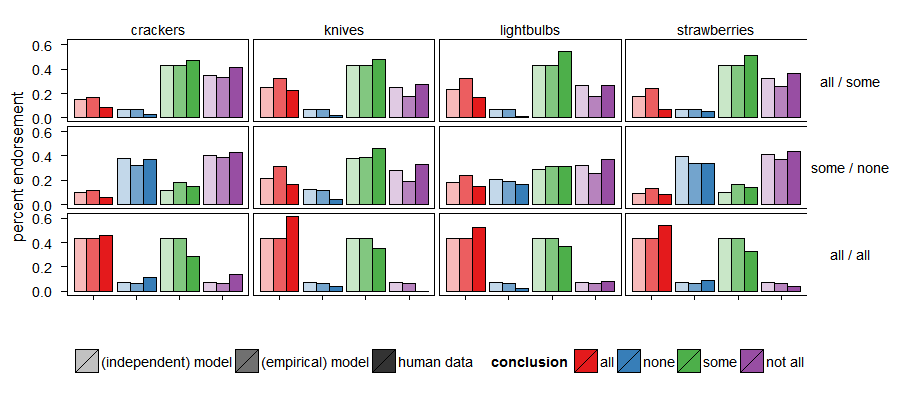
\includegraphics[width=\columnwidth]{figures/bars}
    \caption{Reasoning patterns and predictions for 3 (of the 8) syllogisms in the experiment. Human reasoning data is in the darkest shade. The lighest shade is the 12-parameter (``independent'') model. The medium shade is the 0-parameter (``empirical prior'') model. All syllogisms shown here were of the form B-A / C-B and the conclusions were of the form C-A (e.g. First row: All B are A, Some C are B). Reasoning effects can be seen by comparing rows within a column. Content effects can be seen by comparing columns within a row.}
  \label{fig:syllogismXdomain}
\end{figure}

This modeling work reveals that the empirical prior model predicts the data well. Using Bayesian data analytic techniques, I observed that the 4-parameter ``iid'' model and the 12-paramter ``independent'' model can also accommodate the content effects well. I say the models \emph{accomodate} the data because their predictions are dependent on the particular parameter settings inferred \emph{from that data}. The empirical prior model, by contrast, predicts the data with no parameter fitting. Additionally, it's likely that performing a formal, Bayesian model comparison between these models would favor the empirical prior model due to Bayes' Occam's Razor. However, it is interesting to consider that the implications of these modeling results as they stand. 

The 4-parameter ``iid'' model is the simplest model that could possibly account for content effects. What this model posits is that there is some difference in the base rate of properties in these four different domains. In terms of cognition, this might mean that our artificial domains (e.g. knives that could be sharp, rusty, and/or that cut well) call to mind a general intuition about the base rate of these properties, and that this general base rate enters into the computation of argument strength. The posterior over base rate parameters for this model is consistent with this explanation: base rates for domains with properties that tended to co-occur (e.g. the lightbulbs domain) were relatively high while those for domains with properties that tended \emph{not} to co-occur (e.g. the crackers domain) were low.

The 12-parameter ``independent'' model also accommodates the data. This model posits that properties are independent but differ in their base rates. Correlations between properties don't need to be tracked explicitly. 

An alternative explanation for the ubiquitous good fits is that the experiment itself is confounded. The 8 syllogisms used in my experiment might not be the best syllogisms to distinguish models with subtly different assumptions about the priors over properties. Further, it may also be the case that categorical syllogistic reasoning at large might not be the best experiment to distinguish between these models. In categorical syllogisms, there are only 3 logical possibilities for conclusions entailed by situations: all, some and not all, or none. It's possible that these models would make different predictions if we allowed more possible responses, e.g. most and few.

Finally, it is worth noting that classical reasoning experiments such as the one explored here use language to communicate information for participants to reason over. Basic communicative principles, however, are often neglected in the scientist's analysis of behavior. TG formalized basic communicative principles in their probabilistic pragmatics model of syllogistic reasoning, as an extension of the Rational Speech-Act theory of language understanding. I leave for future work the interplay between pragmatics and prior beliefs in the syllogistic domain. 



%This work highlights the importance of taking into account these communicative principles as well how prior beliefs are integrated into the reasoning process. Recent work has demonstrated how violations of these communicative principles can result in behavior inconsistent with rational models of communication \cite{Degen2015submitted}. Further work will investigate how and where rational integration of prior beliefs breaks 

%\subsection{Wonky worlds?}
%\section{Conclusion}

\bibliographystyle{apacite}
\small{
\bibliography{belief}}

\end{document}
